\documentclass[tikz, margin=0.25mm]{standalone}

\begin{document}
    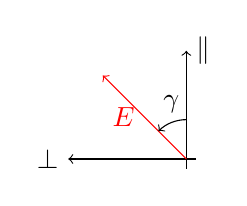
\begin{tikzpicture}
    %axis
        \draw[->]   (0.125,0) -- (-1.5,0) node[left] {$\bot$} ;
        \draw[->] (0,-.125) -- +(0,1.5) node[right] {$\parallel$};
    %result
    \draw[->, red] (0,0) -- (135:1.5) node[midway,left]{$E$};
    \draw[->] (0,0.5) arc (90:135:.5) node[midway,above]{$\gamma$};
    % \node[draw,below,right](ar) at (0.125,-0.5) {$a_r=A\cos(\phi)$};
    % \node[draw,above,left](br) at (-0.125,1) {$b_r=A\sin(\phi)$};
    \end{tikzpicture}  
\end{document}